\documentclass{article}
\usepackage{bera}
\usepackage{listings}
\usepackage{xcolor}
\usepackage{graphicx}
\usepackage{float}


\colorlet{punct}{red!60!black}
\definecolor{background}{HTML}{EEEEEE}
\definecolor{delim}{RGB}{20,105,176}
\colorlet{numb}{magenta!60!black}

\lstdefinelanguage{json}{
    basicstyle=\normalfont\ttfamily,
    numbers=left,
    numberstyle=\scriptsize,
    stepnumber=1,
    numbersep=8pt,
    showstringspaces=false,
    breaklines=true,
    frame=lines,
    backgroundcolor=\color{background},
    literate=
     *{0}{{{\color{numb}0}}}{1}
      {1}{{{\color{numb}1}}}{1}
      {2}{{{\color{numb}2}}}{1}
      {3}{{{\color{numb}3}}}{1}
      {4}{{{\color{numb}4}}}{1}
      {5}{{{\color{numb}5}}}{1}
      {6}{{{\color{numb}6}}}{1}
      {7}{{{\color{numb}7}}}{1}
      {8}{{{\color{numb}8}}}{1}
      {9}{{{\color{numb}9}}}{1}
      {:}{{{\color{punct}{:}}}}{1}
      {,}{{{\color{punct}{,}}}}{1}
      {\{}{{{\color{delim}{\{}}}}{1}
      {\}}{{{\color{delim}{\}}}}}{1}
      {[}{{{\color{delim}{[}}}}{1}
      {]}{{{\color{delim}{]}}}}{1},
}



\begin{titlepage}
   \begin{center}
       \vspace*{1cm}
       
       \textbf{\LARGE Master Thesis - SeEDS (Secure and Efficient Data Namespace) }
       
       \vspace{1.5cm}
       \textbf{Author: Fotios Bistas, fot.bistas@aueb.gr}
       
       \textbf{Advisor: George Xylomenos, xgeorge@aueb.gr}
       
       \textbf{Reviewer: Vasilios Siris, vsiris@aueb.gr}
       
       \textbf{Reviewer: George Polyzos, polyzos@aueb.gr}

       \vspace{0.8cm}
            
       Department Name: Computer Science\\
       University Name: Athens University of Economics and Business\\
       Country: Greece\\
       Date: October 2025
       
       \vspace{0.8cm}

        
\includegraphics[width=0.9\textwidth]{images/opa.png}
   \end{center}
\end{titlepage}

\begin{document}

\section{Introduction}

A \textit{Data Space}, in the sense defined by ETSI ( European Telecommunications Standard Institute ), is a standards-based way
for many independent organizations to make their data discoverable and usable
to one another while each party keeps control of its own data. Instead of
moving everything into one central database, participants adopt common formats,
interfaces, and policies (identity, consent, usage rules) so they can share
data securely and auditably across organizational boundaries. This model aims
to break down today’s “data silos” ( isolated collections of data that prevent data sharing ) and enable new services that combine data
from multiple sources.

This differs from proprietary Content Delivery Networks (CDNs). CDNs focus on
fast distribution of static content (e.g., web assets, video) through
infrastructure operated by a single provider. In contrast, a Data Space
prioritizes interoperability, governance, and data sovereignty across many
owners, rather than speed of delivery from one centralized platform.

We have already implemented a simple Data Space based on the \textit{Named Data Networking (NDN)} architecture, in our previous project \textit{NGI Sargasso OC1 SNDS}. Named Data Networking (NDN) is a data-centric networking paradigm that shifts communication from host-based addressing (as in IP networks) to content-based addressing. In NDN, data are identified and retrieved directly by \textit{names} rather than by the location of the host that stores them. Each piece of data is cryptographically signed by its producer, ensuring authenticity and integrity regardless of where it is fetched from. This enables efficient in-network caching, data reuse, and intrinsic security properties that align naturally with the decentralized and self-sovereign principles of Data Spaces. Consequently, NDN networks are particularly well-suited for environments where multiple parties exchange data without relying on centralized servers or trusted intermediaries. Utilizing the NDN the system supported advanced data-driven applications over a fully distributed and self-sovereign identity framework.

Building upon SNDS, the \textit{Secure and Efficient Data Spaces (SeEDS)} project aims to deliver an ETSI-compliant Data Space solution. The project provides implementations for all required data API operations, including content filtering based on user-defined conditions, as well as optional temporal API operations that enable long-term data storage and retrieval. Specifically, this thesis implements the following goals regarding SeEDS:

\begin{itemize}
    \item Implement the full NGSI-LD API, including content filtering, temporal operations and event subscriptions.  
    \item Enhance data space efficiency by providing distributed data intermediaries and migrating content filters to their optimal location.
    \item Test the SeEDS implementation over the worldwide NDN testbed. 
\end{itemize}

The NGSI-LD API is a standardized interface for managing and exchanging
\emph{context information} in data spaces, as specified by ETSI. It provides a
common, HTTP-based framework that lets content providers, consumers, and
brokering services create, update, and query \emph{entities}, as well as
subscribe to change events. In NGSI-LD, each entity is represented in JSON-LD
and usually consists of a globally unique \texttt{id}, a \texttt{type} (its class),
and a set of \emph{attributes}. Attributes are either \emph{Properties} (values,
optionally with metadata such as \texttt{observedAt} or \texttt{unitCode}) or
\emph{Relationships} (links to other entities). A JSON-LD \texttt{@context}
binds the terms used to well-defined IRIs, ensuring semantic interoperability.

\begin{lstlisting}[language=json, caption={Example JSON-LD},label={lst:ngsi-ld-json}]
{ 
"@id": "urn:seeds:Car:001,
"@type": "Car,
"brand":{
    "type": "Property,
    "value": "BW
},
"dateVehicleFirstRegistered": { 
    "type": "Property
    "value": "201
    "emissionsCO2":{
        "type": "Property,
        "value": "2
    }
},
"@context":[
    "https://example.com/context.jsonl
] 
} 
\end{lstlisting}

This enables SeEDS to support two retrieval modes over its HTTP API: by \texttt{@id} and by \texttt{@type}.
A \emph{GET by ID} request retrieves a single JSON-LD entity given its globally
unique \texttt{@id}. A \emph{GET by TYPE} request retrieves all entities that
match the provided \texttt{@type}. Since \texttt{@type} is optional in SeEDS,
entities that omit it are treated as having the default \texttt{GENERIC} type.

\noindent\textbf{HTTP usage}
\begin{itemize}
  \item \textbf{GET by ID}: returns one entity
  \begin{verbatim}
  GET /?id=urn:seeds:car:car001
  \end{verbatim}

  \item \textbf{GET by TYPE}: returns an array of entities
  \begin{verbatim}
  GET /?type=Vehicle
  \end{verbatim}

  \item \textbf{Implicit type (default)}: entities without @type are treated as
  \texttt{GENERIC}
  \begin{verbatim}
  GET /?type=GENERIC
  \end{verbatim}
\end{itemize}

\noindent\textbf{Response shape}
\begin{itemize}
  \item GET by ID $\rightarrow$ a single JSON-LD object (the entity).
  \item GET by TYPE $\rightarrow$ a JSON array of JSON-LD entities.
\end{itemize}

\section{Architecture}

SeEDS bridges IP and NDN networks via two interfaces. First, it offers an
HTTP endpoint for exchanging NGSI-LD API messages with IP-based systems.
Second, it connects to the NDN Forwarding Daemon (NFD) through a netlink
socket to exchange NDN-specific messages with NDN nodes. Also each SeEDS Service contains a storage instance, where it stores data like locally published IDs, subscribed Nodes etc. The aforementioned are the components of the SeEDS Service. RV ( Rendezvous ) Nodes are nodes that can aggregate content and serve collections of it when queried to.

\begin{figure}[H]
    \centering
    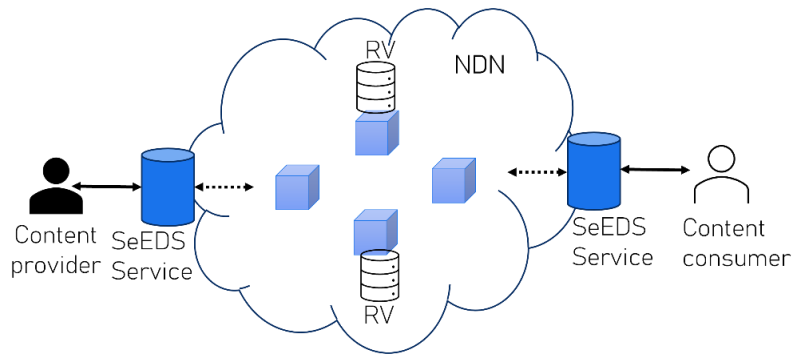
\includegraphics[width=0.8\linewidth]{images/seeds_architecture.png}
    \caption{High level SeEDS architecture.}
    \label{fig:seeds_architecture}
\end{figure}

\pagebreak

The following is the SeEDS Service components in detail: 

\begin{figure}[H]
    \centering
    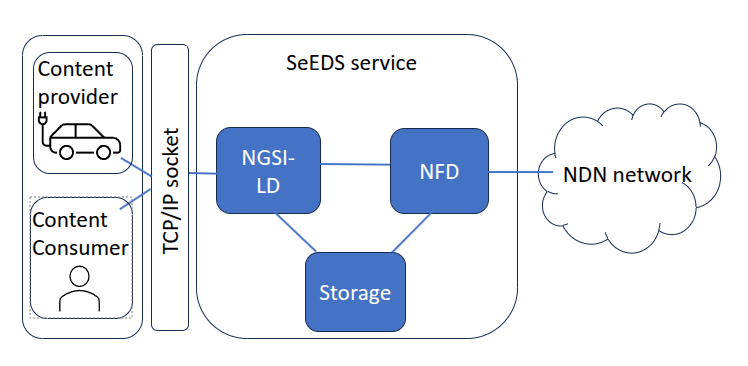
\includegraphics[width=0.8\linewidth]{images/seeds_service_detail.png}
    \caption{SeEDS Service in detail.}
    \label{fig:seeds_service_detail}
\end{figure}

The current architecture enables the SeEDS Service to perform the following operations: 

\begin{itemize}
    \item Consumers can create a \textit{HTTP GET} request to retrieve items from the NDN network. As mentioned before these are either \emph{GET by TYPE} or {GET by ID}. Note that the \textit{@type} and \textit{@id} need to be provided accordingly. 
    \item Providers can create \textit{HTTP POST} requests to provide/announce items to the NDN network. The service will also ensure that the data is stored inside its storage, ensuring that the data can be served when requested from some other node in the network. 
    \item Clients can also subscribe to a specific \textit{@id} or \textit{@type}. Since content in NDN is retrieved by its unique name rather than by host address, clients may express a request for a name even before the corresponding data is available. Once the data is published under that name, the network delivers it to all subscribed clients, enabling efficient and timely notifications.
    \item The NDN naming scheme also enables any NDN node to act as a \emph{Secondary} for another node within the network. A \emph{Secondary} node inherits the data of its corresponding \emph{Primary} node, including its storage contents, announced \textit{@ids}, \textit{@types} and \textit{subscriptions}. This design enhances the resilience of the SeEDS system, allowing it to recover the data of a failed node seamlessly and maintain service continuity.
\end{itemize}

\section{Implementation}

\subsection{GET by ID}

\subsection{GET by TYPE}

\subsection{SUBSCRIPTIONS by ID}

\subsection{SUBSCRIPTIONS by TYPE}

\subsection{Temporal Queries}

\subsection{Resilience}

\section{Experiments}

\section{Conclusion}

\end{document}
